\section{Introduction}
%Brief	introduction	of	the	overall	setting
The goal of this project is to design control parameters for motor-mass-spring fourth order SIMO (Single Input Multiple Output) system. First of all it is important to understand the physical components of the system and which sensor and actuator are present.

A input signal (current, A) is applied to a motor(object 1) which will turn a spring which is connected to a mass which rotates (object 2). Both objects have encoders and are used to close the loop of the control system, acting as feedback. A few more values are affect the systems like inertia (shape), torque, value of mass, spring characteristic and friction.

This assignment is not only designing control parameters but also interfering with a simulator for the plant. The simulator acts not as a continuous systems but a discrete system with sampling period of 100 $\mu$s. This has to be taken into account during the design in order to. The simulator is a FPGA running xlinux like many high-end FPGAs.

This plant is shown in Figure \ref{fig:plant} along with the tasks and how the they connect to it through the communication bus. Then Figure \ref{fig:task} shows how the tasks connect to together within a TDM frame and their slots. In this figure there are four tasks allowed thereof the three tasks, sensing, computing and actuating. These task and their execution within the TDM frame and its various size will be one of the main topics of this reports. These two figures are taken from the assignments slides.

\begin{figure}[h]
	\begin{center}
		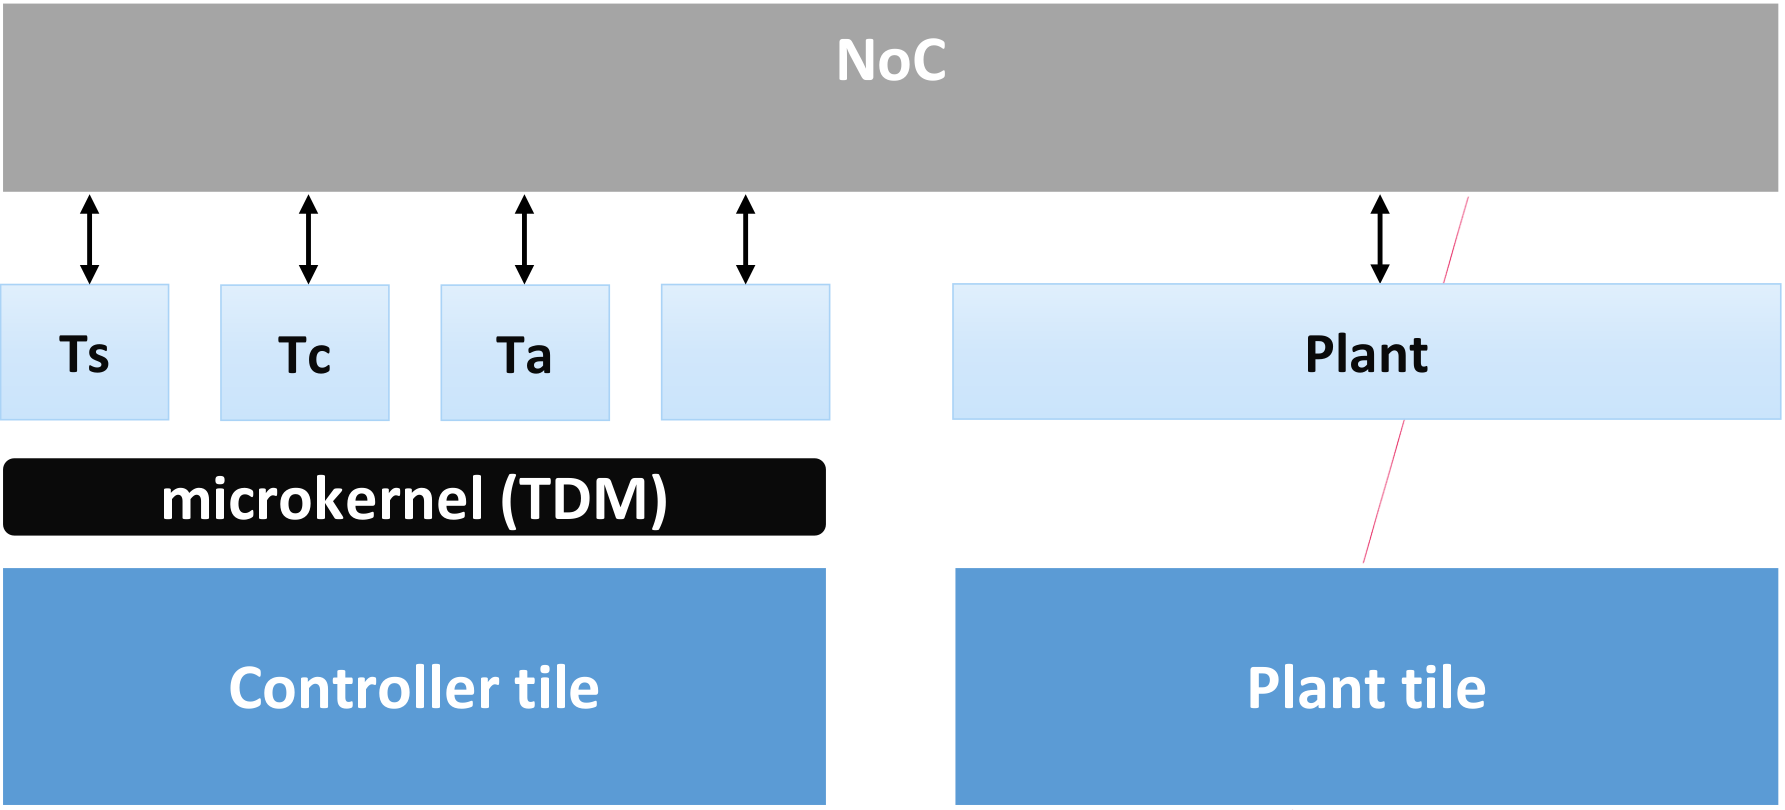
\includegraphics[width=0.7\linewidth]{img/plant}
		\caption{Task Schedule on the platform}.
		\label{fig:plant}
	\end{center}
\end{figure}

\begin{figure}[h]
	\begin{center}
		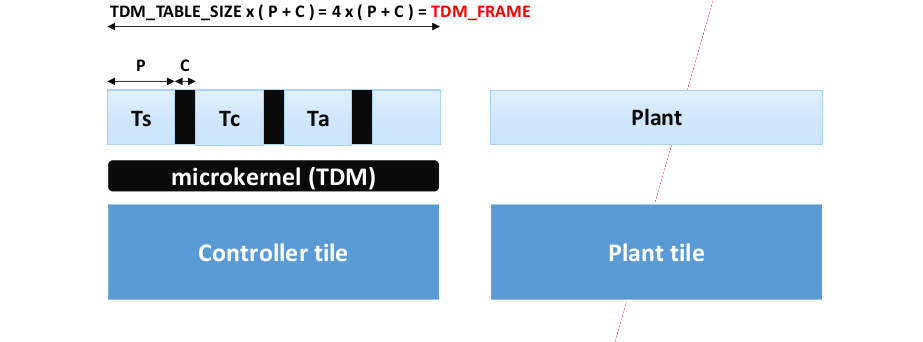
\includegraphics[width=0.7\linewidth]{img/task}
		\caption{Partition of Task Frame to slots}.
		\label{fig:task}
	\end{center}
\end{figure}




